\subsection{Energieübertragung}\label{sec:energieuebertragung}
Mit Hilfe des Induktionsprinzips wird der Dōjō geladen und zwar ohne, dass dieser angeschlossen oder in einer anderen Form vorbereitet werden muss. Dank der induktiven Ladeschaltung, erfolgt der Ladezyklus sobald der Dōjō in die dafür vorgesehene Ladebuchse eingeführt wird. Im folgenden Abschnitt wird die genaue Funktionsweise der Induktionsladeschaltung vorgestellt und analysiert:

\subsubsection*{Grundlegendes}
Beim Induktionsladeprinzip wird Energie mithilfe von Spulen über eine kurze Distanz zwischen zwei Schaltungen transportiert. Die erste Schaltung, von welcher aus die Energie gesendet wird, wird Transceiver genannt. Diese Schaltung besteht im Grundsatz aus einem Pulsgenerator, mit welchem das LC-Glied gepulst wird. Sie macht den Hauptanteil einer solchen Induktiven Ladeschaltung aus. Die zweite, kleinere Schaltung, welche die Energie des Transceivers empfängt, wird Receiver genannt und besteht ebenfalls aus einem LC-Glied, ergänzt mit einem Gleichrichter.

\subsubsection*{Tranceiver}
Der bereits erwähnte Pulsgenerator wird durch eine Timer-Schaltung erreicht. Verwendet wird hierbei das elektronische Bauelement NE555. Dieses bietet den Vorteil, dass er zum einen einfach einzustellen und andererseits das Pulssignal einfach erstellt werden kann. Der NE555 enthält eine monolithisch integrierte Zeitgeberschaltung, die sich aufgrund ihrer Eigenschaften als Taktgeber, Oszillator und für Zeitverzögerungen verwenden lässt. Das Funktionsprinzip des Timers ist, das mithilfe der extern angeschlossenen Elemente, welche aus Widerständen und Kondensatoren bestehen, verschiedene Spannungsschwellen erreicht werden müssen, bevor der Timer zu schalten beginnt. Dabei können mithilfe unterschiedlicher Verhältnisse der externen Elemente die Pulsdauer, die Frequenz und der Duty cycle eingestellt werden. Das entstehende Pulssignal speist schlussendlich das LC-Glied. Um dies zu ermöglichen wird das LC-Glied an die Versorgungsspannung gehängt und in Serie dazu der Collectoranschluss eines Leistungs NPN-Transistor angeschlossen. An dessen Emitter wird nun ein Niederohmiger Widerstand auf GND gehängt, wobei die über ihm abfallenden Spannung von einem weiteren Transistor überwacht wird und somit den Strom begrenzt. Dieser \glqq Strombegrenzungs-Transistor\grqq wird zwischen dem Pulssignal, welches den Leistungs-Transistor steuert, und GND gehängt. Wird nun der Strom und somit auch die Spannung über dem Widerstand zu hoch so schliesst der \glqq Strombegrenzungs-Transistor\grqq das Pulssignal kurz. Der Leistungstransistor wird nicht mehr sauber durchgesteuert und der Strom wird begrenzt. Die Strombegrenzung ist abhängig, welche Teile für das LC-Glied verwendet werden. Es ist darauf zu achten, welches der Beiden Elemente (LC-Glied/Leistungstransistor) weniger Strom verträgt. In diesem Fall ist dies die Spule, welche aufgrund ihrer geringen Baugrösse nur einen Strom von 1.1 A verträgt. Würden grössere Spulen verwendet, so ist eine Begrenzung von 15A notwendig, da dies die Belastungsgrenze für den Leistungstransistor ist.
\newline
Das Pulssignal selber muss verschiedene Kriterien erfüllen. Zum einen sollte der Duty Cycle so nahe wie möglich an 50$\%$ sein. Um dies zu erreichen muss somit gelten: R2 >> R1. Das andere Kriterium ist, das die Resonanzfrequenz des LC-Gliedes getroffen werden sollte. Um das Pulssignal einzustellen, können folgende Richtlinien betrachtet werden:


\begin{description}
	\item [$\cdot$ C] beeinflusst die Zeiten (Frequenz/High-Time/Low-Time)
	\item [$\cdot$ R$_{1}$] beeinflusst die High-Time, lässt jedoch die Low-Time unverändert.
	\item [$\cdot$ R$_{2}$ ] beeinflusst die High- und Low-Time und beeinflusst somit den Duty Cycle.
\end{description}

Die exakte Berechnung lässt sich wie folgt beschreiben:
 \newline
: \newline
: \newline
Em Joscha sini Berechnig vo de Dimensionierig vo de Bauteili
 \newline
: \newline
: \newline
 \newline

Nachdem nun die grobe Frequenz berechnet wurde, können die Elemente ausgesucht und eingebaut werden. Es ist zu beachte, dass Abweichungen sich unmittelbar auf die Frequenz des Pulssignales wie auch auf den Duty Cycle auswirken. Eine solche Abweichung kann bereits durch eine leicht abweichende Resonanzfrequenz des LC-Gliedes auftreten.
\newline
Speziell ist, dass für die Energieübertragung als Sender- und Empfängerspule das selbe LC-Glied verwendet wurde. Dies wurde so gewählt, da das Energiefeld sehr klein ist und im Falle einer grösseren Spule das Receiver Glied nicht optimal ausgenutzt werden könnte. Wie der Receiver aufgebaut ist, wird im nachfolgenden Abschnitt genauer erläutert.

\subsubsection*{Receiver}
Der Receiver besteht primär aus einem LC-Glied und einem Gleichrichter. Für die Spule des LC-Gliedes wurde eine kleine Flachspule verwendet, welche eine Dimension von 15mm Durchmesser und 2mm Höhe aufweist, und somit im inneren des Dōjō’s am Boden montiert werden kann. Der notwendige Kondensator für die Vervollständigung des LC-Gliedes kann direkt hinter der Spule montiert werden. Die hochfrequente Wechselspannung welche nun gemessen werden kann, muss für die Speisung der Batterie noch gleichgerichtet werden. Verwendet werden hierbei sowhl Kondensatoren als auch spezielle Gleichrichterdioden, welche eine Abfallspannung von lediglich 0.1 V aufweisen. Anschliessend wird die gesamte Ladeschaltung gespiesen, welche den gesamten Ladeprozess des Akkus übernimmt. Einen Einblick in den gesamten Ladeprozess gibt das Kapitel \ref{sec:energiespeicher}.


\subsubsection*{Ladestation}

Nachdem die gesamte induktive Ladeschaltung beschrieben wurde, folgt die Beschreibung der Ladestation. Hierfür wurde ein Prototyp erstellt, welche zum einen die gesamte primäre induktive Ladeschaltung beinhaltet, zum anderen eine Aussparung, welche als Ladeeinrichtung für den Dōjō dient, vorweist. Für den Prototypen wurde eine .stl Datei erstellt welche mit einem 3D-Drucker gedruckt wurde. Wichtig ist hierbei zu erwähnen, dass es sich bei nachfolgende Abbildungen \ref{fig:Prototyp Front} bis \ref{fig:Prototyp Down} nur um Prototypen handelt und es bei einer Weiterentwicklung noch Anpassungen geben kann. Da die Ladestation für Versuchszwecke betreffend der induktiven Ladeschaltung bereits erstellt wurde, ist das Design so gewählt, dass nur ein Dōjō geladen werden kann. Dies könnte in einem weiteren Schritt auf mehrere Ladeaussparungen erweitert werden, wobei mehrere Dōjōs gleichzeitig pro Ladestation geladen werden können. 

\begin{figure}[H]
	\begin{center}
		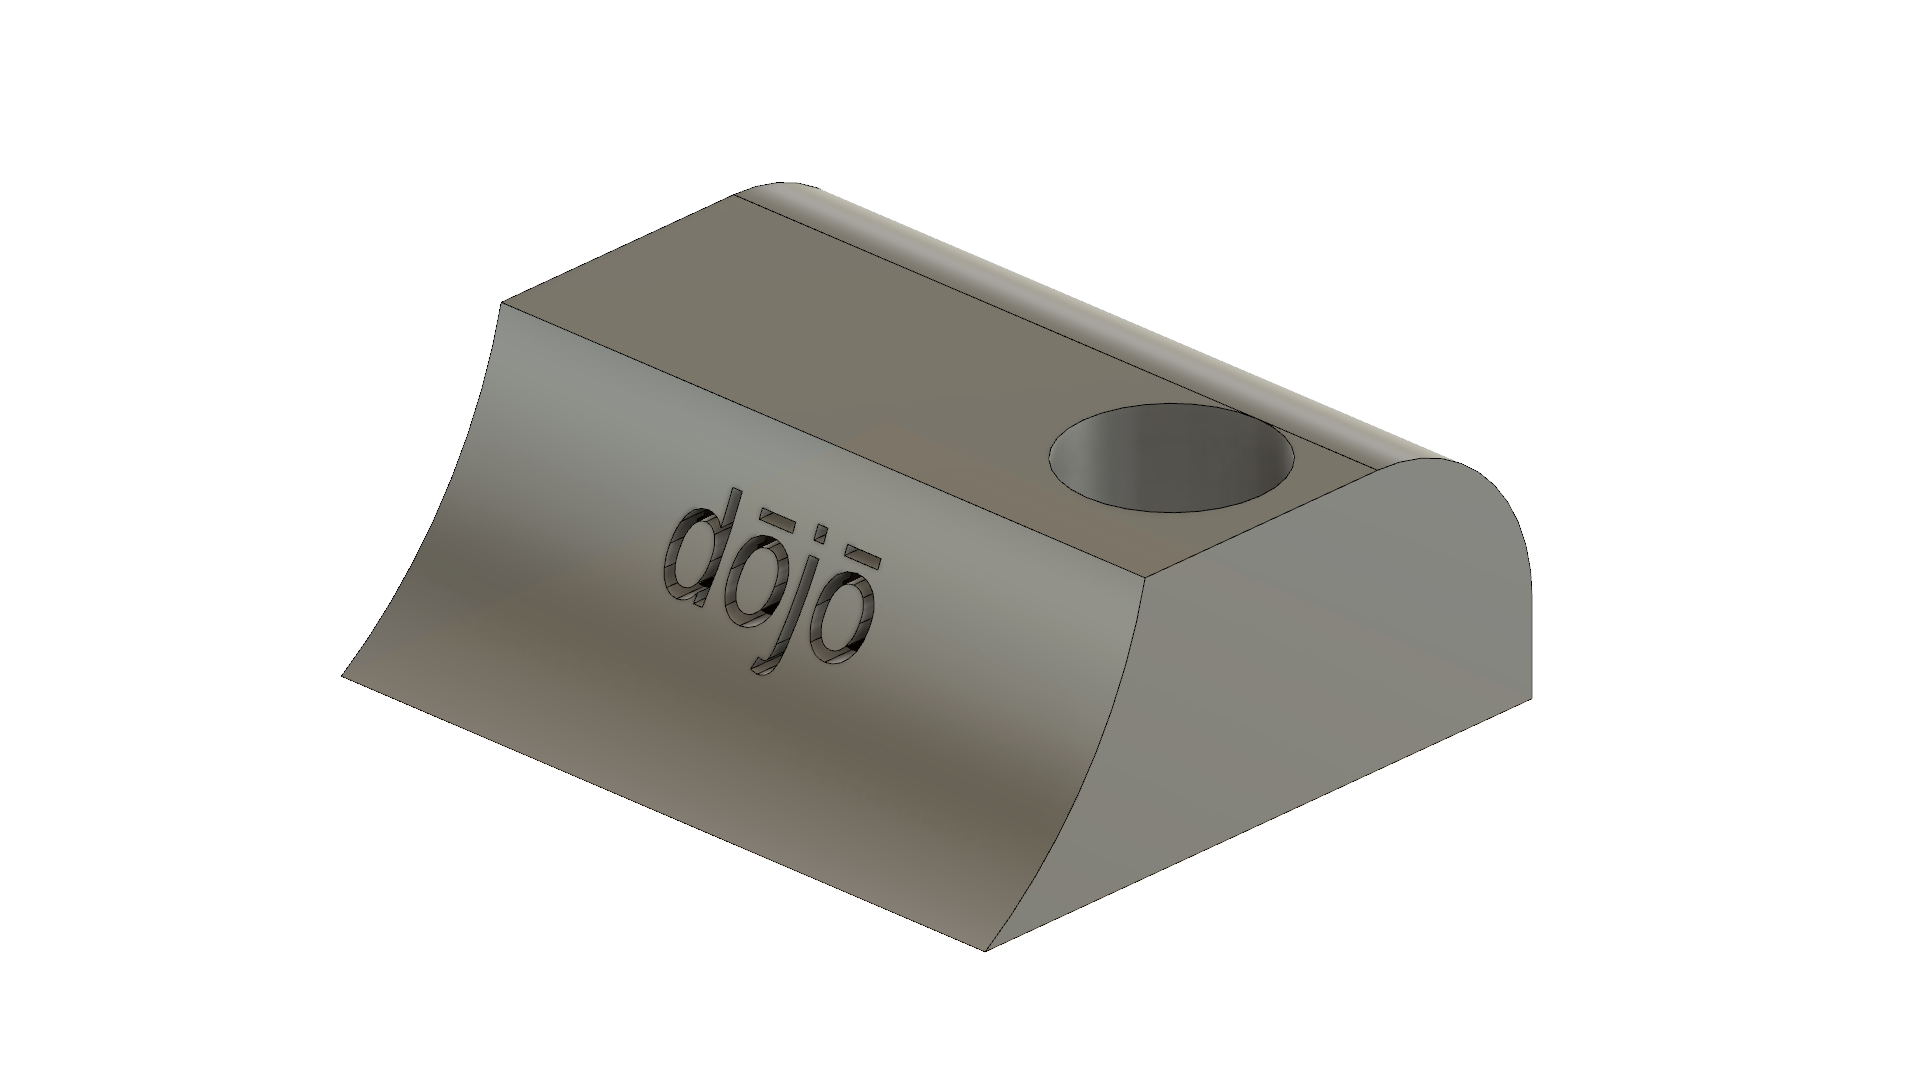
\includegraphics[width=80mm]{data/DojoLadestation01.png}
		\caption[Prototyp Ladestation Frontansicht]{Frontansicht - Ladestation Dōjō} %picture caption
		\label{fig:Prototyp Front}
	\end{center}
\end{figure}

Die oben gezeigte Abbildung gibt einen Einblick in das Design von vorne. Augenfällig ist die Öffnung für den Dōjō selbst, welche zum einen als Standhalterung und zum anderen als korrekte Positionierung für die induktive Ladeschaltung dient. Die richtige Positionierung ist hierbei eines der wichtigsten Kriterien für einen optimalen Ladezyklus, da die Tranceiver- und Receiverspule direkt übereinanderliegend den besten Wirkungsgrad erzielen. Weiter ist in der Abbildung der Dōjō Schriftzug ersichtlich, welcher bis in die dahinter liegende Kammer führt. Die Verwendung dieser Durchführung wird nachfolgend unter der Abbildung \ref{fig:Prototyp Down} weiter erklärt. 


\begin{figure}[H]
	\begin{center}
		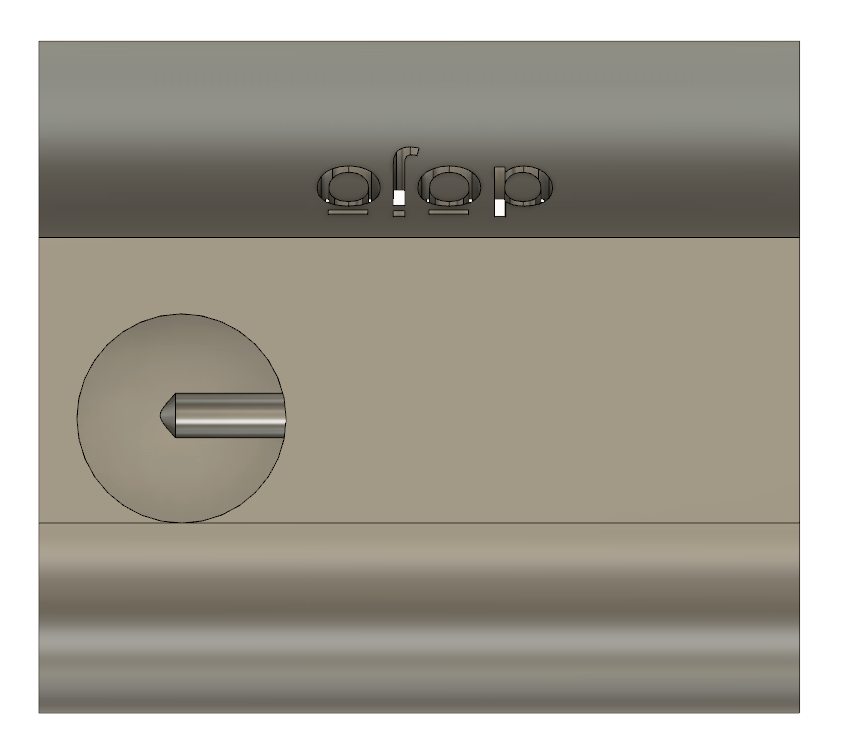
\includegraphics[width=80mm]{data/DojoLadestation02.png}
		\caption[Prototyp Ladestation Draufsicht]{Draufsicht - Ladestation Dōjō} %picture caption
		\label{fig:Prototyp Top}
	\end{center}
\end{figure}

Die obige Abbildung \real{fig: Prototyp Top} zeigt den Prototypen von oben. In der Aussparung für den Dōjō ist ein Kanal für die Verkabelung der Primärspule ersichtlich. Diese Öffnung führt zur Kammer welche den Primär-Ladekreises beinhaltet. Die Abmessung (Länge x Breite x Höhe) des Prototypen ist (80 x 70.7 x 30)mm. Einen Einblick in die Kammer für die Elektronik des Primär-Ladekreises gibt nachfolgende Abbildung \ref{fig:Prototyp Down}, welche den Prototypen von unten zeigt.

\begin{figure}[H]
	\begin{center}
		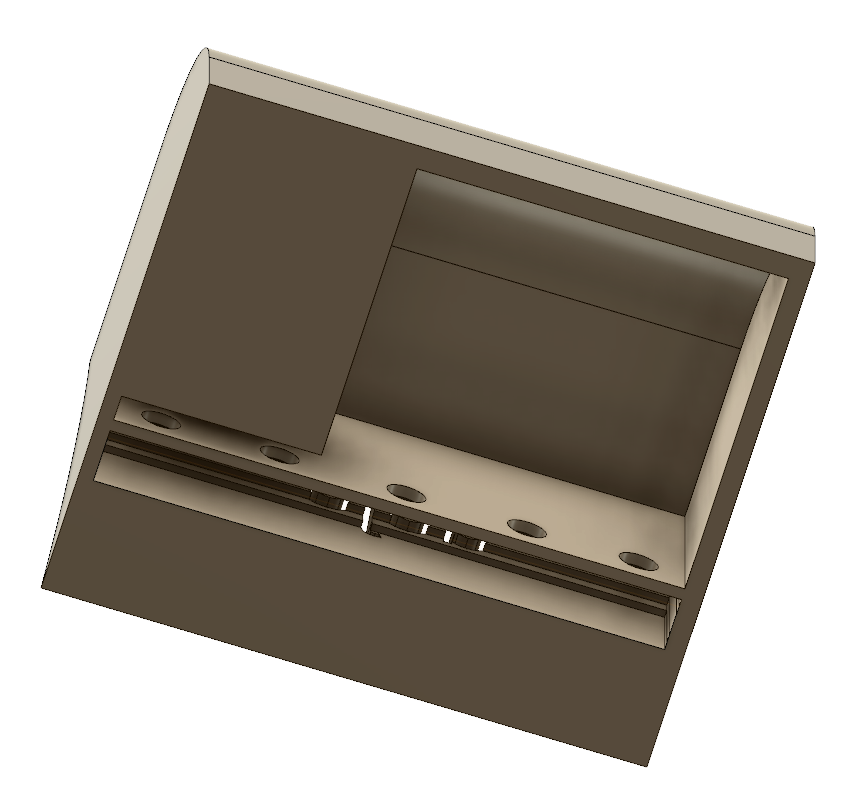
\includegraphics[width=80mm]{data/DojoLadestation03.png}
		\caption[Prototyp Ladestation Ansicht von Unten]{Ansicht von Unten - Ladestation Dōjō} %picture caption
		\label{fig:Prototyp Down}
	\end{center}
\end{figure}

Die grosse Kammer ist wie bereits oben beschrieben für den Primärkreis der induktiven Ladeschaltung vorgesehen. Für die ersten Tests wurde eine Lochrasterplatine mit allen nötigen Komponenten gefertigt, welche genau in diese Aussparung passt. Weiter sind runde Löcher (5mm $\o$) ersichtlich welche in die Kammer des Schriftzuges führen ersichtlich. Diese Durchführungen sind für LED vorgesehen, welche den Dōjō Schriftzug bei angeschlossener Versorgungsspannung zum Leuchten bringt. 